\vfill 
\chapter{Réalisation}
\label{chap:conception}
\vfill 
\minitoc
\mtcaddchapter
\vfill 

\newpage

\section*{Introduction}
\justifying
Dans le dernier chapitre, nous allons présenter les divers outils et framework employés pour la création de notre application. Ensuite, nous illustrons l'intégration  du modèle LLM pour élucider les requêtes des étudiants et l’évaluation du modèle appliqué. Finalement, nous capturerons  quelques interfaces réalisées de notre plateforme.

\section{Environnement et outils de travail}
\justifying
Dans cette section, nous allons présenter les différents outils matériels et logiciels utilisés pour la mise en œuvre de notre plateforme.
\subsection{Environnement matériel }
Pour mettre en place notre solution, nous avons utilisé deux ordinateurs portables. Le tableau 5.1 illustre leurs caractéristiques.
\begin{longtable}{|c|c|c|}
    \caption{Caractéristiques de l’environnement matériel} \\
    \hline
    & \textbf{Ordinateur 1} & \textbf{Ordinateur 2} \\
    \hline
    \textbf{Marque} & HP & Lenovo \\
    \hline
    \textbf{Processeur} & Intel i7 10\textsuperscript{ème} génération & Intel i5 8\textsuperscript{ème} génération \\
    \hline
    \textbf{Ram} & 12 GO & 8 GO \\
    \hline
    \textbf{Disque Dur} & 512 GO SSD & 512 GO SSD \\
    \hline
    \textbf{Système d’exploitation} & Windows 10 & Kubuntu LTS 22 \\
    \hline
\end{longtable}

\subsection{Environnement logiciel}
Le tableau 5.2 illustre la liste des outils utilisés lors du développement de notre application web. \newpage
\begin{longtable}{|p{4cm}|p{11cm}|}
    \caption{Liste des outils utilisé lors du développement de l’application} \\
    \hline
        \textbf{Outil/Technologie} & \textbf{Description} \\
    \hline
    \centering \textbf{Visual Studio Code} \vspace{0.2cm} \newline \centering 
\includegraphics[width=1.5cm,height=1.5cm]{chp5/vscode.png} & Visual Studio Code est un éditeur de code source développé par Microsoft reconnu pour sa légèreté, sa robustesse et ses extensions. \\
    \hline
    \centering \textbf{Postman} \vspace{0.2cm} \newline \centering 
\includegraphics[width=1.5cm,height=1.5cm]{chp5/postman.png} & Postman est une plateforme de développement API qui permet de créer, tester et déboguer des API de manière efficace. \\
    \hline
    \centering \textbf{Git} \vspace{0.2cm} \newline \centering 
\includegraphics[width=1.5cm,height=1.5cm]{chp5/git.png} & Git est un système de contrôle de version distribué et largement utilisé pour suivre les changements dans le code source. \\
    \hline
    \centering \textbf{GitHub} \vspace{0.2cm} \newline \centering 
\includegraphics[width=1.5cm,height=1.5cm]{chp5/github.png} & GitHub est une plateforme de développement logiciel basée sur Git qui offre des fonctionnalités de collaboration et de gestion de projets. \\
    \hline
    \centering \textbf{Draw.io} \vspace{0.2cm} \newline \centering 
\includegraphics[width=1.5cm,height=1.5cm]{chp5/drawio.png} & Draw.io est un outil de création de diagrammes en ligne qui permet de créer des diagrammes de manière intuitive et collaborative. \\
    \hline
    \centering \textbf{Excalidraw} \vspace{0.2cm} \newline \centering 
\includegraphics[width=1.5cm,height=1.5cm]{chp5/excalidraw.png} & Excalidraw est un outil de prototypage de l'interface utilisateur en ligne qui permet de créer des wireframes de manière simple et rapide. \\
    \hline
    \centering \textbf{React.js} \vspace{0.2cm} \newline \centering 
\includegraphics[width=1.5cm,height=1.5cm]{chp5/reactjs.png} & React.js est une bibliothèque JavaScript pour la création d'interfaces utilisateur interactives et dynamiques. \\
    \hline
    \centering \textbf{Next.js} \vspace{0.2cm} \newline \centering 
\includegraphics[width=2.5cm,height=1.5cm]{chp5/nextjs.png} & Next.js est un framework JavaScript React qui permet de construire des applications web performantes avec une expérience de développement simplifiée. \\
    \hline
    \centering \textbf{Tailwind CSS} \vspace{0.2cm} \newline \centering 
\includegraphics[width=1.5cm,height=1cm]{chp5/tailwind.png} & Tailwind CSS est une bibliothèque CSS utilitaire qui permet de concevoir rapidement des interfaces utilisateur modernes et personnalisées. \\
    \hline
    \centering \textbf{Prisma} \vspace{0.2cm} \newline \centering 
\includegraphics[width=1.5cm,height=1.5cm]{chp5/prisma.png} & Prisma est un ORM (Object-Relational Mapping) qui facilite l'interaction avec la base de données en utilisant un langage de requête TypeScript sécurisé. \\
    \hline
    \centering \textbf{PostgreSQL} \vspace{0.2cm} \newline \centering 
\includegraphics[width=1.5cm,height=1.5cm]{chp5/postgresql.png} & PostgreSQL est un système de gestion de base de données relationnelles robuste et performant. \\
    \hline
    \centering \textbf{Supabase} \vspace{0.2cm} \newline \centering 
\includegraphics[width=1.5cm,height=1.5cm]{chp5/supabase.png} & Supabase est une plateforme de développement intégrée qui offre une base de données PostgreSQL hébergée et d'autres fonctionnalités de backend. \\
    \hline
    \centering \textbf{Node.js} \vspace{0.2cm} \newline \centering 
\includegraphics[width=1.5cm,height=1.5cm]{chp5/nodejs.png} & Node.js est un environnement d'exécution JavaScript côté serveur qui permet d'exécuter du code JavaScript en dehors du navigateur. \\
    \hline
    \centering \textbf{TypeScript} \vspace{0.2cm} \newline \centering 
\includegraphics[width=1.5cm,height=1.5cm]{chp5/typescript.png} & TypeScript est un langage basé sur JavaScript développé par Microsoft avec un typage statique optionnel. Il facilite la détection précoce et la correction des erreurs lors du développement. \\
    \hline
    \centering \textbf{Vercel} \vspace{0.2cm} \newline \centering 
\includegraphics[width=1.5cm,height=1.5cm]{chp5/vercel.jpg} & Vercel est une plateforme de déploiement qui permet de déployer des applications frontend et backend de manière rapide, simple et évolutive. \\
    \hline
    \centering \textbf{Langchain} \vspace{0.2cm} \newline \centering 
\includegraphics[width=1.5cm,height=1.5cm]{chp5/langchain.png} & Langchain est un framework développé dans le but de faciliter la création d'applications en utilisant des grands modèles de langage (LLM). \\
    \hline
    \centering \textbf{Pinecone} \vspace{0.2cm} \newline \centering 
\includegraphics[width=1.5cm,height=1.5cm]{chp5/pinecone.png} & Pinecone est une base de données vectorielle qui offre une infrastructure efficace pour stocker et manipuler des données vectorielles. \\
    \hline
\end{longtable}

\section{Framework Next.js}
Notre application web est développée en utilisant le framework Next.js qui est construit sur la bibliothèque ReactJS et qui offre des fonctionnalités supplémentaires pour la création d'applications web modernes. Next.js est un framework full stack qui permet de créer des applications web performantes et optimisées en facilitant la création d'interfaces utilisateur.\\
Avec Next.js, nous pouvons utiliser le dossier \textbf{"app"} pour gérer le routage de notre application. Il permet de créer des routes dynamiques, des groupes de routes et des routes imbriquées en créant simplement des dossiers.\\
La Figure 5.1 illustre la structure du dossier \textbf{“app”}.\\


\noindent En outre, Next.js offre également un dossier spécial appelé \textbf{"api"} pour créer des endpoints API pour la partie backend de notre application.\\
Cela permet de créer facilement des API REST pour notre application.\\
De plus, il est important de noter que Next.js propose également les \textbf{"Server Actions"} qui peuvent également jouer un role rôle similaire à celui du dossier \textbf{"api"} pour créer des endpoints API.\\
Les Figures 5.2 et 5.3 illustrent la structure des dossiers \textbf{“api”} et \textbf{“actions”}.\\



\noindent Next.js simplifie ainsi la création d'applications web full stack en fournissant une solution complète pour la gestion du routage et de la création d'API.




\section{Intègration du Modèle LLM}
Dans cette section, nous allons présenter l'intégration de l'API GroqCloud, les étapes d'élucidation des documents, ainsi que l'évaluation du modèle.
\subsection{API GroqCloud}
Dans notre plateforme, nous avons mis en œuvre le modèle Mixtrel of Experts (MoE) pour répondre à nos besoins en utilisant l'API de Groq, une société américaine spécialisée dans l'intelligence artificielle qui développe un accélérateur d'IA circuit intégré spécifique à l'application sous le nom de \textbf{L}anguage \textbf{P}rocessing \textbf{U}nit \textbf{(LPU)}. Cette API nous permet d'accéder aux différentes fonctionnalités du modèle MoE afin de créer un chatbot interactif capable de répondre aux questions des étudiants en se basant sur le contexte des documents partagés par eux-mêmes ou par leurs enseignants ainsi que sur des ressources externes. Cette fonctionnalité permettra aux étudiants d'obtenir des réponses rapides et précises à leurs questions et d'améliorer leur expérience utilisateur sur notre plateforme.\\
La figure 5.4 illustre l'intégration de l'API de Groq dans notre plateforme.
\begin{figure}[H]
    \centering
    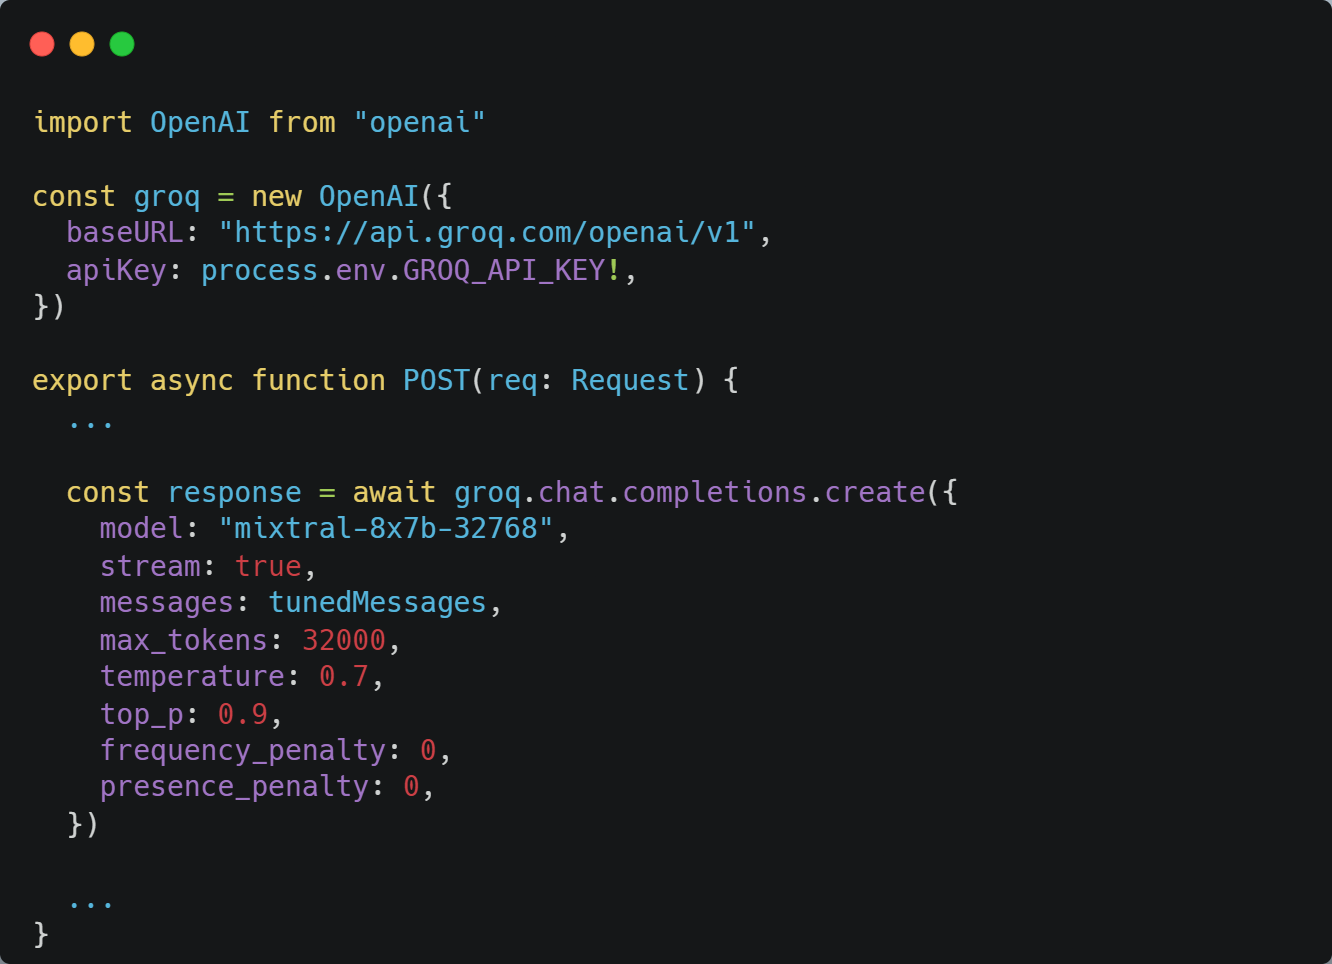
\includegraphics[width=\textwidth]{images/chp5/fig4.png}
    \caption{Intégration de l'API GroqCloud dans notre plateforme}
    \label{fig:Integration de l'API GroqCloud dans notre plateforme}    
\end{figure}
\subsection{Etapes}
La Figure 5.5 synthétise les étapes et le fonctionnement de Dynamic RAG pour la génération de réponses précises et pertinentes en illustrant un exemple de requête pour un étudiant.\\
Cette approche s'appuie sur l'utilisation de l'API GroqCloud ainsi que sur l'intégration d'autres technologies.
\begin{figure}[H]
    \centering
    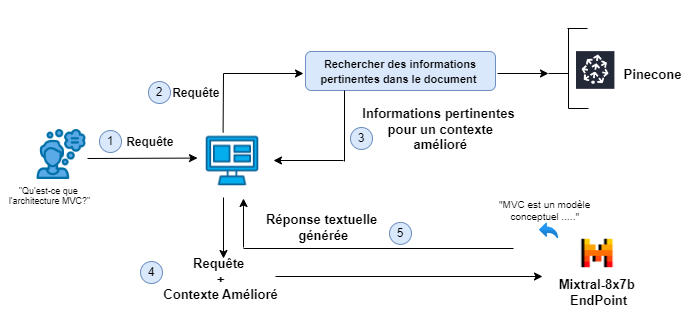
\includegraphics[width=\textwidth]{images/chp5/fig5.png}
    \caption{Exemple du déroulement et des étapes de Dynamic RAG avec nos technologies}
    \label{fig:Exemple du déroulement et des étapes de Dynamic RAG avec nos technologies}
\end{figure}

\subsection{Evaluation}
Étant donné que nous avons appliqué  le modèle Mixtral 8x7b via l'intégration de l’API GroqCloud qui déjà évaluée et validée.  Nous ne sommes pas, donc, en mesure d'effectuer une évaluation du modèle par nous-mêmes ,mais, nous allons nous focaliser sur des métriques d'évaluations standards qui nous semblent pertinentes dans le contexte de notre travail. En particulier, nous avons mis le focus sur les cinq métriques d'évaluation suivantes :
\begin{itemize}
    \item \textbf{Qualité}: La qualité est une métrique qui mesure la précision et la fiabilité des résultats produits par le modèle. Elle permet d'évaluer la performance du modèle en termes de pertinence et de cohérence des réponses fournies.
    \item \textbf{Vitesse}: La vitesse est une métrique qui mesure le temps nécessaire pour qu'un modèle de langage traite une requête et génère une réponse.
    \item \textbf{Latence}: La latence est le temps nécessaire pour qu'un système réponde à une demande ou à une entrée. Dans le contexte des modèles de langage, la latence se réfère au temps nécessaire pour que le modèle traite une requête et génère le premier token de la réponse.
    \item \textbf{Fenêtre de contexte}: La fenêtre de contexte est une métrique qui mesure la quantité d'informations prises en compte par le modèle pour traiter une requête.
    \item \textbf{Codage}: Le critère de codage dans fait référence à la capacité du modèle à comprendre, interpréter et générer du code informatique.
\end{itemize}
Notons que les informations de cette section sont issues de la référence suivante.[15]

\begin{itemize}
    \item \textbf{Qualité du Mixtral 8x7B }
\end{itemize}
\noindent Le modèle Mixtral 8x7B a obtenu un score \textbf{MMLU} (\textbf{M}assive \textbf{M}ultitask \textbf{L}anguage \textbf{U}nderstanding) de \textbf{0.706} qui reflète sa capacité à comprendre et à traiter le langage naturel dans diverses tâches. De plus, il a un indice de qualité de \textbf{65}. Ce score est le résultat de plusieurs évaluations et montre que le modèle est fiable et performant dans différents contextes d'utilisation. Bien que ces résultats puissent être améliorés, le Mixtral 8x7B reste un modèle compétitif sur le marché et offre une qualité satisfaisante pour de nombreuses applications de traitement automatique du langage naturel.

\begin{itemize}
    \item \textbf{Vitesse du Mixtral 8x7B}
\end{itemize}
\noindent Un des points forts du Mixtral 8x7B réside dans sa rapidité d'exécution. En effet, ce modèle est plus rapide que la moyenne avec un débit impressionnant de \textbf{97,7 tokens par seconde}. Cette caractéristique fait un choix avantageux pour les applications nécessitant une génération rapide de texte.

\begin{itemize}
    \item \textbf{Latence du Mixtral 8x7B }
\end{itemize}
\noindent Le Mixtral 8x7B est remarquable en termes de latence. Avec un temps de réception du premier token (Time to First Token) de seulement \textbf{0,24 seconde}. Cette latence garantit une réactivité accrue du modèle lors de son utilisation et offre ainsi une expérience utilisateur améliorée.

\begin{itemize}
    \item \textbf{Fenêtre de contexte du Mixtral 8x7B }
\end{itemize}
\noindent Le Mixtral 8x7B présente une fenêtre de contexte avec une capacité de \textbf{33 000 tokens}. Cette capacité est en réalité suffisante pour de nombreuses tâches de traitement de langue naturelle. En outre, cette fenêtre de contexte de 33 000 tokens peut être avantageuse pour le traitement de longs documents ou de contextes étendus car elle permet de prendre en compte un contexte plus large que certains modèles concurrents.

\begin{itemize}
    \item \textbf{Codage }
\end{itemize}
\noindent \textbf{HumanEval} : Dans l'évaluation des compétences en codage, le modèle obtient un score de \textbf{40,2}, ce qui est considéré comme un bon résultat. Cela démontre la capacité du modèle à comprendre et à générer du code de manière efficace. [16]

\section{Travail réalisé }
Dans cette section nous allons présenter quelques interfaces de notre plateforme.

\section*{Conclusion}
Dans ce chapitre final, nous avons débuté en présentant les outils logiciels et le matériel que nous avons employés pour la réalisation de notre projet, ainsi que l'intégration du modèle LLM pour. Enfin, nous avons clôturé par quelques interfaces qui présentent les principales fonctionnalités de notre plateforme.
